% main.tex : Post-CFET paper (IEEEtran, two-column) — conference-safe full text

\documentclass[conference]{IEEEtran}

% ---------- Packages ----------
\usepackage{newtxtext,newtxmath}
\usepackage{xcolor}
\usepackage{graphicx}
\usepackage{booktabs}
\usepackage{multirow}
\usepackage{standalone}
\usepackage{gincltex}
\usepackage{tikz}
\usetikzlibrary{positioning,fit,shapes,arrows.meta,mindmap,trees,calc}
\usepackage{siunitx}
\sisetup{per-mode=symbol,range-phrase=\text{--},range-units=single}
\usepackage{url}
\usepackage{hyperref}
\usepackage{placeins}   % \FloatBarrier
\usepackage{balance}    % 段バランス(最終ページ安定)

% ---------- TikZ styles (for roadmap etc.) ----------
\tikzset{
  milestone/.style={circle,draw=red!70,fill=red!60,minimum size=4pt,inner sep=0pt},
  bubble/.style={rectangle,rounded corners=2pt,draw=black!25,fill=white,
                 font=\footnotesize,align=center,inner sep=2pt},
  arrow/.style={-Latex,thick}
}

% ---------- Macros ----------
\newcommand{\figpath}{figures}
\newcommand{\tikzcol}[2][\linewidth]{\resizebox{#1}{!}{\input{#2}}}
\newcommand{\etal}{\textit{et al.}}

% ---------- Title & Author ----------
\title{Post-CFET Device Architectures: Materials, Integration, and Design Perspectives}

\author{
\IEEEauthorblockN{Shinichi Samizo}
\IEEEauthorblockA{Independent Semiconductor Researcher\\
Project Design Hub, Samizo-AITL\\
\textit{Email:} \href{mailto:shin3t72@gmail.com}{shin3t72@gmail.com}\quad
\textit{GitHub:} \href{https://github.com/Samizo-AITL}{Samizo-AITL}}
}

\begin{document}
\maketitle

% ---------- Abstract ----------
\begin{abstract}
CMOS scaling has evolved from planar MOSFETs to FinFETs, Gate-All-Around (GAA) nanosheets and Complementary FETs (CFETs).
While CFET improves electrostatic control and mitigates local wiring bottlenecks, further gains are constrained by material, thermal and reliability limits of silicon.
This paper surveys post-CFET device options---two-dimensional (2D) material FETs, monolithic 3D (M3D) integration, spintronics/quantum devices, and heterogeneous atomic-scale integration.
We discuss their physical principles, process and integration challenges, demonstrated performance, reliability concerns, design/EDA implications, and educational aspects.
A comparison matrix and a 2030--2045 roadmap are provided.
\end{abstract}

% ---------- 1. Introduction ----------
\section{Introduction}
Over five decades, the industry advanced by shrinking devices and re-architecting transistors: Planar $\rightarrow$ FinFET $\rightarrow$ GAA $\rightarrow$ CFET.
Dennard scaling has long broken; beyond \SI{\sim 3}{nm} nodes, \emph{interconnect delay and power density} dominate, and device self-heating and variability constrain further gains.
Wiring RC delay already exceeds intrinsic device delay for many paths; thermal design power densities approach \SI{1}{W/mm^2} in high-performance logic, stressing reliability (BTI, EM) and packaging.
Consequently, progress increasingly relies on \textbf{materials innovation}, \textbf{vertical integration}, and \textbf{alternative state variables} (spin, photon, charge+heat co-design) rather than lateral device scaling alone.
This work positions ``post-CFET'' as that transition and compares four concrete vectors.

% ---------- 2. Evolution ----------
\section{Evolution from CMOS to Post-CFET}
Fig.~\ref{fig:evolution} sketches the pathway from CMOS to post-CFET candidates.

\subsection{Planar MOSFET to FinFET}
Below \SI{45}{nm} gate lengths, short-channel effects (SCE) and junction leakage degraded $SS$ and $I_{off}$.
Tri-gate FinFETs provided stronger gate coupling and reduced SCE, enabling continued voltage scaling and variability control.

\subsection{FinFET to GAA}
To further compress cell height and suppress corner leakage, stacked nanosheets fully surrounded by the gate were introduced.
GAA improves electrostatics and $V_{T}$ tunability, at the cost of increased process complexity (sacrificial layers, release uniformity) and tighter variability control (line-edge roughness, work-function granularity).

\subsection{GAA to CFET}
CFET vertically stacks complementary devices (nFET over pFET or vice versa), improving cell density and reducing local interconnect delay by gate-level vertical proximity.
Key challenges include \emph{thermal budget management}, \emph{alignment of stacked devices}, and \emph{contact/via resistance} between tiers.

\subsection{Beyond CFET}
As wiring dominance and heat density increase, simply stacking silicon devices hits diminishing returns.
Post-CFET options expand along three axes: (i) introduce new channel or functional materials (2D/TMDs), (ii) pursue true \emph{monolithic} 3D integration to shorten interconnects and co-locate memory/logic, and (iii) adopt \emph{non-charge} state variables (spin) and cross-domain fusion (photonics/MEMS/bio).

% ---------- wide figure ----------
\begin{figure*}[!t]
  \centering
  \tikzcol[0.9\textwidth]{\figpath/evolution_tree.tex}
  \caption{Evolution tree: CMOS $\rightarrow$ CFET $\rightarrow$ post-CFET candidates.}
  \label{fig:evolution}
\end{figure*}

% ---------- 3. Technologies ----------
\section{Post-CFET Candidate Technologies}

\subsection{2D Material FETs}
\textbf{Principle:}
Atomically thin semiconductors (e.g., MoS$_2$, WSe$_2$) provide excellent electrostatic control and suppressed short-channel leakage owing to sub-nm body thickness.
Van der Waals interfaces relax lattice matching constraints, enabling heterogeneous stacks.

\textbf{State-of-the-art:}
Lab-scale devices with $L_g\!\sim\!10$--\SI{20}{nm} show $I_{on}/I_{off}\!\sim\!10^7$ and $SS\!\sim\!60$--\SI{70}{mV/dec}.
Contact resistivity remains high ($R_c\!\sim\!0.5$--\SI{1}{k\Omega\cdot\mu m}); wafer-scale CVD growth shows \SI{5}{\%}--\SI{10}{\%} non-uniformity and grain-boundary-induced variability.

\textbf{Integration:}
Low-temperature BEOL-compatible processes (\SI{<450}{^\circ C}) are desired for sequential stacking or CFET+2D hybrids.
Key knobs are phase/defect control, substitutional/charge-transfer doping, metal/TMD interface engineering, and clean transfer (or direct growth) on dielectrics and Cu-compatible liners.

\textbf{Reliability:}
Interface traps, charge trapping/de-trapping, and self-heating through low-$k$ dielectrics impact BTI-like shifts and mobility.
Environmental stability (oxidation, moisture) requires encapsulation (e.g., h-BN, ALD Al$_2$O$_3$).

\textbf{Design/EDA implications:}
Compact models must capture quantum confinement, Schottky contacts, and variability (grain boundaries, thickness steps).
PDKs need parameter corners for $R_c$, mobility, contact asymmetry, and layout rules addressing transfer seams and 2D-specific proximity effects.

\textbf{Applications:}
Ultra-low-power edge nodes, flexible/bio electronics, steep-slope concepts and sensor-logic co-integration.
Near term, 2D devices likely \emph{complement} CFETs (e.g., analog sensing layers atop logic).

\subsection{Monolithic 3D Integration (M3D)}
\textbf{Principle:}
Sequential device fabrication forms multiple active layers on a single wafer with fine-pitch inter-layer vias (ILVs), shortening interconnects by \(\gg\!100\times\) versus 2.5D/TSV stacks.

\textbf{State-of-the-art:}
Demonstrations include 3D SRAM/logic with delay reductions ($\sim$30\%) and area savings ($\sim$40\%), as well as memory-centric AI tiles showing $>\!1.5\times$ system energy efficiency.

\textbf{Integration:}
Main constraints are \textbf{thermal budget} (\SI{<450}{^\circ C} after the first tier), dopant activation at low-$T$, and \textbf{alignment/yield}.
Laser/flash anneal, solid-phase epitaxy, and low-$T$ materials (oxide semiconductors, 2D) are active areas.
ILV pitch $<\SI{200}{nm}$ with acceptable resistance and electromigration margins is a key milestone.

\textbf{Thermal/mechanical:}
Vertical heat flow and local hotspots require thermal-aware placement, TSV/ILV planning, and stress-aware signoff (Coffin--Manson fatigue, wafer bow).

\textbf{Design/EDA implications:}
3D placement \& routing with layer assignment, ILV budgeting, thermal and stress co-simulation, and timing closure that includes vertical parasitics.
Power delivery network (PDN) partitioning across tiers and integrated thermal throttling policies are needed.

\textbf{Applications:}
AI accelerators (near-/in-memory compute), memory-wall mitigation for graph/transformer workloads, and low-latency sensor fusion.

\subsection{Spintronics / Quantum Devices}
\textbf{Principle:}
Magnetic tunnel junctions (MTJs) exploit spin-dependent tunneling (CoFeB/MgO stacks), enabling non-volatile memory (STT/SOT-MRAM) and logic-in-memory concepts.
Quantum/topological devices explore spin--orbit coupling and edge states.

\textbf{State-of-the-art:}
STT-MRAM endurance of $10^{12}$ cycles at room temperature; SOT-MRAM reduces write latency and improves endurance by separating read/write paths, at the expense of area/driver complexity.

\textbf{Integration:}
BEOL-friendly temperatures (\SI{<400}{^\circ C}) are feasible; challenges include write current reduction (mA $\rightarrow$ $\mu$A), variability of $H_k$/$TMR$, and read disturb.
Hybrid stacks (e.g., MRAM over logic tiers in M3D) enable ultra-fast, non-volatile buffers and checkpointing.

\textbf{Design/EDA implications:}
Compact models must include stochastic switching, retention distributions, and temperature dependence.
For compute-in-memory (CIM), EDA flows need array-level analog behavior, error-rate aware mapping, and ECC co-design.

\textbf{Applications:}
Radiation-tolerant systems (space/avionics), last-level cache augmentation, always-on inference, neuromorphic primitives.

\subsection{Heterogeneous Atomic-Scale Integration}
\textbf{Principle:}
Fuse dissimilar domains (Si CMOS + photonics + MEMS + sensors + 2D) by leveraging van der Waals interfaces, direct wafer bonding, or hybrid bonding.

\textbf{State-of-the-art:}
Examples include Si+MoS$_2$ photodetectors (responsivity $\sim\SI{200}{mA/W}$ at \SI{1.55}{\micro m}), CMOS+MEMS inertial sensors, and on-chip photonics for low-latency I/O.

\textbf{Integration:}
Interface cleanliness/planarity, CTE/lattice mismatch, and bonding yield dominate.
Cross-domain verification (optical S-parameters, mechanical eigenmodes) must be integrated with electrical timing and power.

\textbf{Design/EDA implications:}
Compact models spanning domains, co-simulation backplanes (SPICE + FDTD/RCWA + FEM), and PDKs that provide optical/mechanical layer stacks, DRC, and reliability rules.

\textbf{Applications:}
Optical interconnect, medical/industrial sensing, aerospace instruments, and co-packaged optics.

% ---------- 4. Comparison Matrix (two-column safe) ----------
\FloatBarrier
\begin{table*}[!t]
\centering
\caption{Comparison of post-CFET candidates (representative, not exhaustive)}
\label{tab:comparison}
\small
\begin{tabular}{@{}lcccc@{}}
\toprule
Tech. & Demo (rep.) & Bottlenecks & Reliability & Design impact \\
\midrule
2D-FET & $I_{on}/I_{off}\!\sim\!10^7$, $SS\!\sim\!65$ mV/dec &
$R_c$, film uniform. & Traps, self-heat &
New compact models, var. kits \\
M3D & Delay $-30$\%, Area $-40$\% &
$<\!450^\circ$C, ILV $R$ & Hotspots, stress &
3D P\&R, thermal/stress co-sim \\
Spin & MRAM $10^{12}$ cyc &
$I_\mathrm{write}$, $TMR$ var. & Retention, disturb &
Stochastic models, ECC/CIM \\
Hetero & Si+2D PD \SI{200}{mA/W} &
Bonding, CTE mismatch & Interface aging &
Cross-domain EDA/PDK \\
\bottomrule
\end{tabular}
\end{table*}
\FloatBarrier

\section{Comparison and Positioning}
Table~\ref{tab:comparison} contrasts each vector from \emph{device}, \emph{integration}, and \emph{design} angles.
A pragmatic path is hybrid: CFET for density, M3D for distance reduction, spintronics for non-volatility, and 2D materials or photonics for sensing/I/O.
The \emph{system} wins when interconnect energy is minimized and memory/compute locality is maximized.

% ---------- 5. Design / Education ----------
\section{Design and Educational Perspectives}

\subsection{EDA/PDK Requirements}
\begin{itemize}
  \item \textbf{Compact models:} Quantum confinement, Schottky contacts (2D), stochastic switching (spin), thermo--electro--mechanical coupling (M3D/hetero).
  \item \textbf{3D physical design:} Tier-aware floorplanning, ILV budgeting, thermal-aware placement, vertical timing/parasitics extraction.
  \item \textbf{Multi-physics co-simulation:} Electrical--thermal--mechanical--optical closed loops with sign-off criteria (hotspot temp., stress limits, optical loss budgets).
  \item \textbf{Reliability sign-off:} BTI/HCI/EM with temperature gradients, MRAM retention/disturb models, interface aging for bonded stacks.
  \item \textbf{Variability/DFM:} Film thickness, grain boundary density, $R_c$ spread, bonding voids; provide statistical corners and Monte Carlo kits.
\end{itemize}

\subsection{Curriculum and Workforce Development}
Graduate curricula should include: (i) device-to-system co-design, (ii) variability-aware modeling labs, (iii) 3D PDN/thermal projects, (iv) cross-domain capstone (e.g., CMOS+photonics+MEMS).
Industry--academia pilot lines (multi-project wafers, shuttle services) can accelerate translational education.

% ---------- 6. Roadmap ----------
\section{Future Scenarios (2030--2045)}

\noindent\textbf{2030--2035 (TRL 3--4):}
2D-FET/CFET hybrid cells and M3D SRAM/logic pilots; ILV pitch \(\lesssim\)\SI{200}{nm}; MRAM pervasive in caches; first cross-domain PDKs.

\noindent\textbf{2035--2040 (TRL 5--6):}
Sequential 3D logic+memory tiles in AI accelerators; reliable $<\SI{450}{^\circ C}$ flows; SOT-MRAM adoption; wafer-level bonding for photonics/2D stacks.

\noindent\textbf{2040--2045 (TRL 7--8):}
HPC/aerospace systems using non-volatile 3D logic--memory, radiation-hard 2D stacks, and co-packaged optics; cross-domain EDA becomes mainstream.

% ---------- 7. Conclusion ----------
\section{Conclusion}
Post-CFET shifts progress from lateral device scaling to a co-optimized space of materials, vertical integration, and new state variables.
A hybrid trajectory---CFET density, M3D distance reduction, spintronic non-volatility, and heterogeneous fusion---offers the best path to energy-efficient systems.
Success hinges on multi-physics EDA/PDKs, reliability- and variability-aware models, and curricula that train device-to-system engineers.

% ---------- Figures at end ----------
\FloatBarrier

\begin{figure*}[!t]
  \centering
  \tikzcol[0.95\textwidth]{\figpath/block_diagram.tex}
  \caption{Conceptual block diagram of candidate device/integration options.}
  \label{fig:block}
\end{figure*}

% --- Fig.3: mindmap を両段幅&ほぼ全幅で ---
\begin{figure*}[!t]
  \centering
  \resizebox{0.98\textwidth}{!}{% figures/mindmap.tex — clean pro look (no mindmap lib)
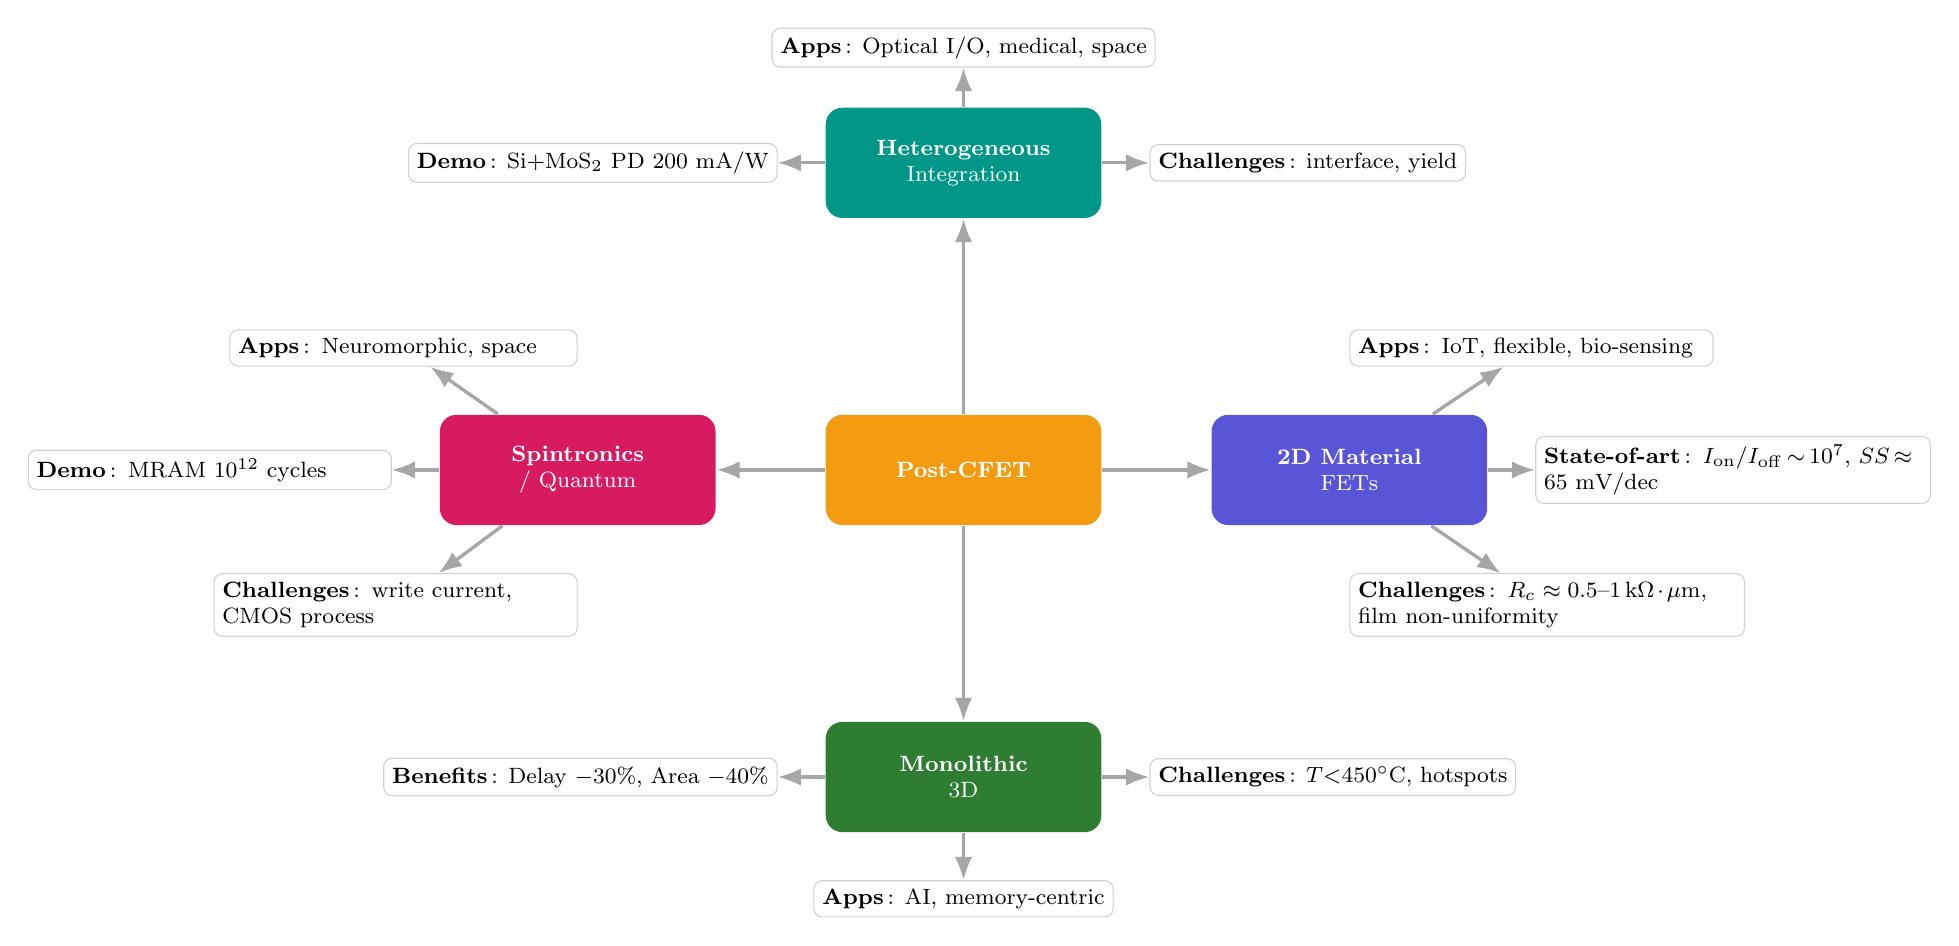
\begin{tikzpicture}[
  %----- styles -----
  font=\footnotesize,
  >=Latex,
  card/.style={
    draw=black!18, rounded corners=3pt, fill=white, align=left,
    inner sep=3pt, minimum width=38mm
  },
  topic/.style={
    rounded corners=6pt, align=center, text=white, semithick,
    minimum width=35mm, minimum height=14mm
  },
  link/.style={-Latex, very thick, draw=black!35},
  dot/.style={circle, fill=black!35, inner sep=1pt}
]
%----- palette (淡色で印刷も可) -----
\definecolor{cCore}{RGB}{243,156,18}   % orange
\definecolor{c2D}{RGB}{88, 86,214}     % blue-violet
\definecolor{cM3D}{RGB}{46,125,50}     % green
\definecolor{cSpin}{RGB}{216,27,96}    % magenta
\definecolor{cHet}{RGB}{0,150,136}     % teal

%----- layout points -----
\node[topic, fill=cCore] (core) at (0,0) {\bfseries Post-CFET};

\node[topic, fill=cHet]  (het)  at (0, 3.9) {\bfseries Heterogeneous\\ Integration};
\node[topic, fill=c2D]   (twod) at (4.9,0) {\bfseries 2D Material\\ FETs};
\node[topic, fill=cM3D]  (m3d)  at (0,-3.9) {\bfseries Monolithic\\ 3D};
\node[topic, fill=cSpin] (spin) at (-4.9,0) {\bfseries Spintronics\\ / Quantum};

% connectors from center
\draw[link] (core) -- (het);
\draw[link] (core) -- (twod);
\draw[link] (core) -- (m3d);
\draw[link] (core) -- (spin);

%----- Heterogeneous cards (top) -----
\node[card, above=5mm of het]   (h-app) {\textbf{Apps}\,: Optical I/O, medical, space};
\node[card, left=6mm  of het]   (h-demo){\textbf{Demo}\,: Si+MoS$_2$ PD 200 mA/W};
\node[card, right=6mm of het]   (h-ch)  {\textbf{Challenges}\,: interface, yield};
\foreach \x in {h-app,h-demo,h-ch} {\draw[link] (het) -- (\x);}

%----- 2D FETs cards (right) -----
\node[card, above=6mm of twod, anchor=south west, text width=44mm] (d-app)
  {\textbf{Apps}\,: IoT, flexible, bio-sensing};
\node[card, right=6mm of twod, anchor=west, text width=48mm] (d-ion)
  {\textbf{State-of-art}\,: $I_{\rm on}/I_{\rm off}\!\sim\!10^7$, $SS\!\approx\!65$ mV/dec};
\node[card, below=6mm of twod, anchor=north west, text width=48mm] (d-ch)
  {\textbf{Challenges}\,: $R_c\!\approx\!0.5$–$1\,\mathrm{k}\Omega\!\cdot\!\mu$m, film non-uniformity};
\foreach \x in {d-app,d-ion,d-ch} {\draw[link] (twod) -- (\x);}

%----- M3D cards (bottom) -----
\node[card, below=6mm of m3d] (m-app) {\textbf{Apps}\,: AI, memory-centric};
\node[card, left=6mm  of m3d] (m-perf){\textbf{Benefits}\,: Delay $-30\%$, Area $-40\%$};
\node[card, right=6mm of m3d] (m-ch)  {\textbf{Challenges}\,: $T{<}450^{\circ}$C, hotspots};
\foreach \x in {m-app,m-perf,m-ch} {\draw[link] (m3d) -- (\x);}

%----- Spin/Quantum cards (left) -----
\node[card, above=6mm of spin, anchor=south east, text width=42mm] (s-app)
  {\textbf{Apps}\,: Neuromorphic, space};
\node[card, left=6mm of spin, anchor=east, text width=44mm]   (s-mram)
  {\textbf{Demo}\,: MRAM $10^{12}$ cycles};
\node[card, below=6mm of spin, anchor=north east, text width=44mm] (s-ch)
  {\textbf{Challenges}\,: write current, CMOS process};
\foreach \x in {s-app,s-mram,s-ch} {\draw[link] (spin) -- (\x);}

% small dots at topic midpoints (飾り)
\foreach \n in {het,twod,m3d,spin} \fill[dot] (\n) circle (0pt);
\end{tikzpicture}
}
  \caption{Post-CFET technology mind map.}
  \label{fig:mindmap}
\end{figure*}

% --- Roadmap 図(通常表示, 文字サイズ固定) ---
\begin{figure*}[!t]
  \centering
  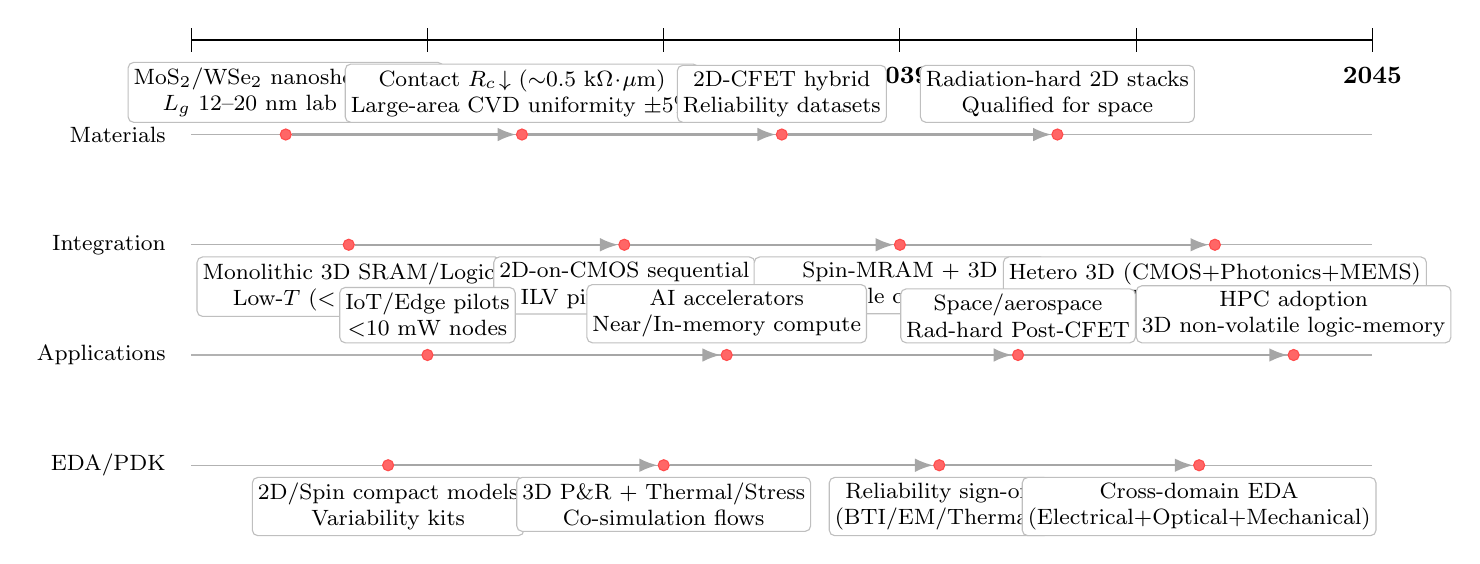
\begin{tikzpicture}[
  >=LaTeX,
  year/.style={font=\bfseries\small},
  lane/.style={font=\footnotesize,align=left}
]
% Axis
\draw[thick] (0,0) -- (15,0);
\foreach \x/\y in {0/2030,3/2033,6/2036,9/2039,12/2042,15/2045} {
  \draw (\x,0.15) -- (\x,-0.15) node[below=2pt,year] {\y};
}

% Lanes
\node[lane, anchor=east] at (-0.2, -1.2) {Materials};
\node[lane, anchor=east] at (-0.2, -2.6) {Integration};
\node[lane, anchor=east] at (-0.2, -4.0) {Applications};
\node[lane, anchor=east] at (-0.2, -5.4) {EDA/PDK};
\draw[gray!60] (0,-1.2) -- (15,-1.2);
\draw[gray!60] (0,-2.6) -- (15,-2.6);
\draw[gray!60] (0,-4.0) -- (15,-4.0);
\draw[gray!60] (0,-5.4) -- (15,-5.4);

% Milestones + bubbles
\node[milestone] (m1) at (1.2,-1.2) {};
\node[bubble, above=2pt of m1] {MoS$_2$/WSe$_2$ nanosheet FETs \\ $L_g$ 12--20 nm lab demos};
\node[milestone] (m2) at (4.2,-1.2) {};
\node[bubble, above=2pt of m2] {Contact $R_c\!\downarrow$ ($\sim$0.5 k$\Omega\!\cdot\!\mu$m) \\ Large-area CVD uniformity $\pm$5\%};
\node[milestone] (m3) at (7.5,-1.2) {};
\node[bubble, above=2pt of m3] {2D-CFET hybrid \\ Reliability datasets};
\node[milestone] (m4) at (11.0,-1.2) {};
\node[bubble, above=2pt of m4] {Radiation-hard 2D stacks \\ Qualified for space};

\node[milestone] (i1) at (2.0,-2.6) {};
\node[bubble, below=2pt of i1] {Monolithic 3D SRAM/Logic \\ Low-$T$ ($<450^\circ$C) flow};
\node[milestone] (i2) at (5.5,-2.6) {};
\node[bubble, below=2pt of i2] {2D-on-CMOS sequential \\ ILV pitch $<$ 200 nm};
\node[milestone] (i3) at (9.0,-2.6) {};
\node[bubble, below=2pt of i3] {Spin-MRAM + 3D \\ Non-volatile compute stack};
\node[milestone] (i4) at (13.0,-2.6) {};
\node[bubble, below=2pt of i4] {Hetero 3D (CMOS+Photonics+MEMS) \\ Production lines};

\node[milestone] (a1) at (3.0,-4.0) {};
\node[bubble, above=2pt of a1] {IoT/Edge pilots \\ $<$10 mW nodes};
\node[milestone] (a2) at (6.8,-4.0) {};
\node[bubble, above=2pt of a2] {AI accelerators \\ Near/In-memory compute};
\node[milestone] (a3) at (10.5,-4.0) {};
\node[bubble, above=2pt of a3] {Space/aerospace \\ Rad-hard Post-CFET};
\node[milestone] (a4) at (14.0,-4.0) {};
\node[bubble, above=2pt of a4] {HPC adoption \\ 3D non-volatile logic-memory};

\node[milestone] (e1) at (2.5,-5.4) {};
\node[bubble, below=2pt of e1] {2D/Spin compact models \\ Variability kits};
\node[milestone] (e2) at (6.0,-5.4) {};
\node[bubble, below=2pt of e2] {3D P\&R + Thermal/Stress \\ Co-simulation flows};
\node[milestone] (e3) at (9.5,-5.4) {};
\node[bubble, below=2pt of e3] {Reliability sign-off \\ (BTI/EM/Thermal)};
\node[milestone] (e4) at (12.8,-5.4) {};
\node[bubble, below=2pt of e4] {Cross-domain EDA \\ (Electrical+Optical+Mechanical)};

\draw[arrow, gray!70] (m1) -- (m2); \draw[arrow, gray!70] (m2) -- (m3); \draw[arrow, gray!70] (m3) -- (m4);
\draw[arrow, gray!70] (i1) -- (i2); \draw[arrow, gray!70] (i2) -- (i3); \draw[arrow, gray!70] (i3) -- (i4);
\draw[arrow, gray!70] (a1) -- (a2); \draw[arrow, gray!70] (a2) -- (a3); \draw[arrow, gray!70] (a3) -- (a4);
\draw[arrow, gray!70] (e1) -- (e2); \draw[arrow, gray!70] (e2) -- (e3); \draw[arrow, gray!70] (e3) -- (e4);
\end{tikzpicture}
% ← そのまま入力(拡大・縮小しない)
  \caption{2030–2045 roadmap (materials, integration, applications, EDA).}
  \label{fig:roadmap}
\end{figure*}

% ---------- References ----------
\balance % 段バランスをここで発動
\begin{thebibliography}{1}
\bibitem{irds2024} IRDS, \emph{International Roadmap for Devices and Systems}, 2024.
\bibitem{takagi2023} S. Takagi, \etal, IEDM Tech Digest, 2023.
\bibitem{liu2022} Z. Liu, \etal, \emph{Nature Electronics}, 2022.
\bibitem{ferr2019} A. Fert, \etal, \emph{Rev. Mod. Phys.}, 2019.
\bibitem{wong2020} H. S. P. Wong, \emph{Nat. Rev. Mater.}, 2020.
\bibitem{batude2019} P. Batude, \etal, IEDM, 2019.
\end{thebibliography}

% ---------- Author Biography (conference-safe, non-float) ----------
\section*{Author Biography}
\textbf{Shinichi Samizo} received the M.S. degree in Electrical and Electronic Engineering from Shinshu University, Japan.
He worked at Seiko Epson Corporation on semiconductor memory and mixed-signal device development and contributed to inkjet MEMS actuators and PrecisionCore printhead technology.
He is currently an independent semiconductor researcher focusing on process/device education, memory architecture, and AI system integration.\\
\emph{Contact:} \href{mailto:shin3t72@gmail.com}{shin3t72@gmail.com}\quad
\emph{GitHub:} \href{https://github.com/Samizo-AITL}{Samizo-AITL}.

\end{document}
